\section{Введение}

\textbf{Цель работы:}
исследовать вынужденную прецессию гироскопа; установить зависимость
скорости вынужденной прецессии от величины момента сил, действующих
на ось гироскопа; определить скорость вращения ротора гироскопа и
сравнить ее со скоростью, рассчитанной по скорости прецессии.


\textbf{В работе используются:}
гироскоп в кардановом подвесе, секундомер, набор грузов,
отдельный ротор гироскопа, цилиндр известной массы, крутильный
маятник, штангенциркуль, линейка.


Уравнения движения твердого тела можно записать в виде:
\begin{equation}
    \frac{d\vec{P}}{dt} = \vec F
\end{equation}
\begin{equation}
    \frac{d\vec L}{dt} = \vec M
\end{equation}

Здесь (1) выражает закон движения центра мас тела, а (2) -
уравнение моментов. Поскольку твердое тело имеет только шесть
степеней свободы, этих двух векторных уравнений достаточно для
полного описания состояния его движения.
\begin{wrapfigure}{r}{0.5\linewidth} % l - слева, r - справа, с - центр
\centering %выравнивание по центру
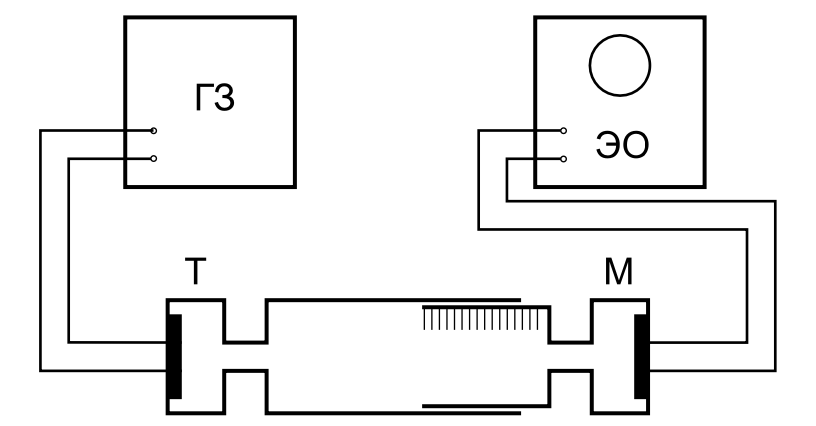
\includegraphics[width=0.5\linewidth,center]{p1.png}
\caption{Маховик} % подрисуночная подпись
\label{pic:my} %метка для ссылки по тексту
\end{wrapfigure}

Если сила $\vec F$ не зависит от угловой скорости, а момент
$\vec M$ - от скорости поступательного движения, то уравнения (1)
и (2) можно рассматривать независимо друг от друга. В баллистике,
например при движении снаряда в воздухе, это невозможно. В случае
же, когда такое раздельное рассмотрение возможно, уравнение (1)
соответствует просто задаче о движении материальной точки, а
уравнение (2) - задаче о вращении твердого тела вокруг неподвижной
точки. В данной работе рассматривается последняя из этих задач.

Момент импульса твердого тела в его главных осях $x, y, z$ равен
\begin{equation}
    \vec L = \vec iI_x\omega_x + \vec jI_y\omega_y + \vec kI_z\omega_z,
\end{equation}

где $I_x, I_y, I_z$ - главные моменты инерции
$\omega_x, \omega_y \omega_z$ -— компоненты вектора угловой
скорости $\vec\omega$. Быстро вращающееся тело, для которого,
например,
\begin{equation*}
    I_z\omega_z \gg I_x\omega_x, I_y\omega_y,
\end{equation*}

принято называть гироскопом. Гироскоп называется уравновешенным,
если его центр масс неподвижен.

В силу (2) приращение момента импульса определяется интегралом
\begin{equation}
    \Delta\vec{L} =\int\vec{M}dt.
\end{equation}

Если момент внешних сил действует в течение короткого промежутка
времени, из интеграла (4) следует, что приращение $\Delta\vec{L}$
момента импульса значительно меньше самого момента импульса:
\begin{equation*}
    |\Delta\vec{L}| \ll |\vec{L}|.
\end{equation*}


С этим связана замечательная устойчивость, которую приобретает
движение гироскопа после приведения его вбыстрое вращение. Выясним,
какие силы надо приложить к гироскопу, чтобы изменить направление
его оси. Рассмотрим для примера маховик, вращающийся вокруг оси $z$
перпендикулярной кплоскости маховика (рис. 1). Будем считать, что
\begin{equation*}
    \omega_z = \omega_0,\text{     }\omega_x = 0,\text{     }\omega_y = 0.
\end{equation*}
Пусть ось вращения повернулась в плоскости $zx$ по направлению к
оси $x$ на бесконечно малый угол др. Такой поворот означает
добавочное вращение маховика вокруг оси $y$, так что
\begin{equation*}
    d\varphi = \Omega dt,
\end{equation*}
где $\Omega$ - угловая скорость такого вращения. Будем
предполагать, что
\begin{equation}
    L_\Omega \ll L_{\omega_0}.
\end{equation}

Это означает, что момент импульса маховика. равный $I_z\omega_0$
до приложения внешних сил, только повернется в плоскости $zx$ по
направлению к оси $x$ не изменяя своей величины. Таким образом,
\begin{equation*}
    |d\vec{L}| = Ld\varphi = L\Omega dt.
\end{equation*}

Но это изменение направлено вдоль оси $x$, поэтому вектор $d\vec{L}$
можно представить в виде векторного произведения вектора угловой
скорости $\Omega$, направленного вдоль оси $y$, на вектор
собственного момента импульса маховика, направленного вдоль оси $z$,
\begin{equation*}
    \frac{d\vec{L}}{dt} = \left[\vec \Omega, \vec L\right]
\end{equation*}
т.е.
\begin{equation}
    \vec{M} = \left[\vec \Omega, \vec L\right]
\end{equation}

Формула (6) справедлива, если выполнено условие (5). Она позволяет
определить момент сил М, который необходимо приложить к маховику
для того, чтобы вызвать вращение оси маховика с угловой скоростью
$\Omega$. Мы видим, таким образом, что для поворота оси
вращающегося маховика к оси $x$ необходимо приложить силы, направденные
не вдоль сои $x$, а вдоль оси $y$, так чтобы их момент $\vec{M}$
был направлен вдоль оси $x$.


Под действием момента $\vec{M}$ внешних сил ось гироскопа медленно
вращается вокруг оси $y$ с угловой скоростью $\Omega$. Такое
движение называется регулярной прецессией гироскопа. В частности,
создающей момент внешней силой может оказаться сила тяжести, если
центр масс гироскопа не совпадает с точкой подвеса. Для гироскопа
массой $m_\text{г}$, у которого ось собственного вращения наклонена
на угол а от вертикали, скорость прецессии, происходящей вокруг
вертикальной оси под действием силы тяжести, равна
\begin{equation}
    \Omega = \frac{M}{I_z\omega_0\sin\alpha} = \frac{m_\text{г}gl_\text{ц}}{I_z\omega_0}
\end{equation}

где $l_\text{ц}$ - расстояние от точки подвеса до центра масс
гироскопа, т.е. скорость прецессии не зависит от угла $\alpha$. Для
изучения регулярной прецессии уравновешенного гироскопа к его оси
подвешивают дополнительные грузы. Это смещает общий центр масс и
создает момент сил тяжести, вызывающий прецессию. Скорость
прецессии в этом случае равна
\begin{equation}
    \Omega =\frac{mgl}{I_z\omega_0},
\end{equation}
где $m$ - масса груза, $l$ — расстояние от центра карданова
подвеса до точки крепления груза на оси гироскопа (рис. 3).

В данной работе исследуется регулярная прецессия уравновешенного
гироскопа.

Уравновешенный гироскоп, закрепленный в кольцах карданова подвеса,
показан на рис. 2. Наружное кольцо подвеса А может свободно
поворачиваться вокруг вертикальной оси аа. Внутреннее кольцо Б
связано с кольцом А горизонтальной ось бб. В кольце Б укреплен
гироскоп, ось вращения которого вв перпендикулярна к оси бб. Центр
масс гироскопа находится на пересечении всех трех осей и при любом
повороте колец сохраняет свое положение в пространстве. Получается,
что гироскоп как бы подвешен за центр масс.

Экспериментальная установка для иследования прецессии
уравновешенного гироскопа показана на рис. 3. Ротором гироскопа
является ротор высокооборотного электромотора М, питающегося током
частотой 400 Гц. Кожух мотора (статор, имеюший обмотки, питаемые
током частотой 400 Гц) скреплен с кольцом Б (рис. 2 и 3). Мотор с
кольцом Б может вращаться в кольце А вокруг горизонтальной оси бб,
которое может вращаться вокруг вертикальной оси аа. Ротор
электромотора представляет массивный стальной цилиндр с прожилками
меди, образующими «беличье колесо». Обозначенный на рис. З буквой
С рычат направлен по оси симметрии ротора. На рычаг подвешивают
грузы Г. Подвешивая различные грузы, можно менять силу $F$, момент
которой определяется расстоянием $l$ от точки подвеса до
горизонтальной оси кольца А (до центра масс гироскопа), указанным
на самой установке.
\begin{figure}[H]
    \centering
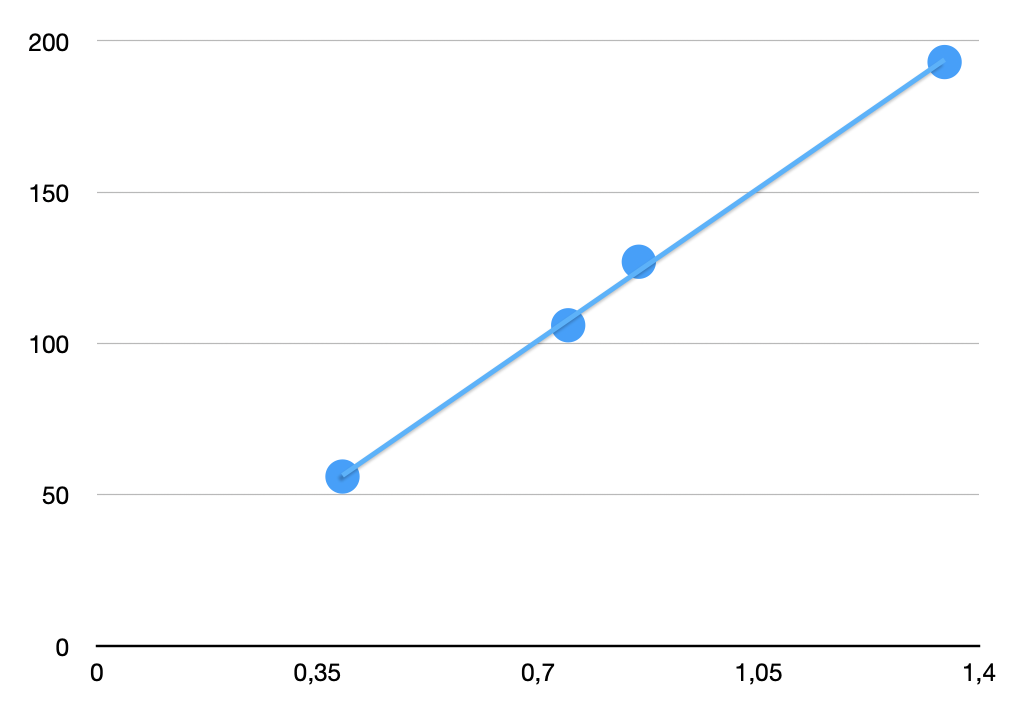
\includegraphics[width=0.4\linewidth,center]{p2.png}
    \caption{Гироскоп в кардановом подвесе}
    \label{fig:my_label}
\end{figure}

Выше при выводе формул для прецессии предполагалось, что
действующие на гироскоп силы лежат в плоскости $zy$, в которой
лежат векторы угловых скоростей собственного вращения и прецессии.
В этом случае, как уже говорилось, момент сил меняет лишь
направление момента импульса гироскопа, но не его величину. Силы
трения не лежат в плоскости осей вращения. Они приводят к изменению
момента импульса и по направлению, и по величине. Для ротора
гироскопа действие сил трения скомпенсировано действием
электромотора. Для осей карданова подвеса компенсации нет. В
результате ось гироскопа будет опускаться в направлении действия
груза. Читателю предлагается проанализировать роль сил трения и
оценить погрешности, которые возникнут при определении скорости
вращения гироскопа относительно его оси симметрии $\omega_0$,
связанные с постепенным опусканием оси гироскопа.

В первой части работы исследуется зависимость скорости прецессии
гироскопа от момента силы, приложенной к его оси. Для этого к оси
гироскопа (к рычагу С) подвешиваются грузы Г. Скорость прецессии
определяется по числу оборотов рычага вокруг вертикальной оси и
времени, которое на это ушло, определяемое секундомером. В процессе
измерений рычаг не только поворачивается в результате прецессии
гироскопа, но и опускается. Поэтому его в начале опыта следует
приподнять на $5-6^\circ$. Опыт надо закончить, когда рычаг
опустится на такой же угол.

Измерение скорости прецессии гироскопа позволяет вычислить угловую
скорость вращения его ротора. Расчет производится по формуле (8).
Момент инерции ротора относительно оси симметрии $I_0$ измеряется
по крутильным колебаниям точной копии ротора, подвешиваемой вдоль
оси симметрии на жесткой проволоке. Период крутильных колебаний $T_0$
зависит от момента инерции $I_0$ и модуля кручения проволоки $f$:
\begin{equation}
    T_0 = 2\pi\sqrt{\frac{I_0}{f}}.
\end{equation}

Чтобы исключить модуль кручения проволоки, вместо ротора гироскопа
к той же проволоке подвешивают цилиндр правильной формы с
известными размерами и массой, для которого легко можно вычислить
момент инерции $I_{\text{ц}}$. Для определения момента инерции
ротора гироскопа имеем
\begin{equation}
    I_0 = I_\text{ц}\frac{T_0^2}{T_\text{ц}^2}
\end{equation}
здесь $T_\text{ц}$ — период крутильных колебаний цилиндра.

Скорость вращения ротора гироскопа можно определить и не прибегая
к исследованию прецессии. У используемых в работе гироскопов статор
имеет две обмотки, необходимые для быстрой раскрутки гироскопа.
В данной работе одну обмотку используют лдя раскрутки тироскопа,
а вторую - для измерения числа оборотов ротора. Ротор электромотора
всегда немного намагничен. Врашаясь, он наводит во второй обмотке
переменную электродвижущую силу (ЭДС) индукции, частота которой
равна частоте вращения ротора. Частоту этой ЭДС можно, в частности,
измерить по фигурам Лиссажу, получаемым на экране осциллографа,
если на один вход подать исследуемую ЭДС, а на другой — переменное
напряжение с хорошо прокалиброванного генератора. При совпадении
частот на экране получаем эллипс.
\begin{figure}[H]
    \centering
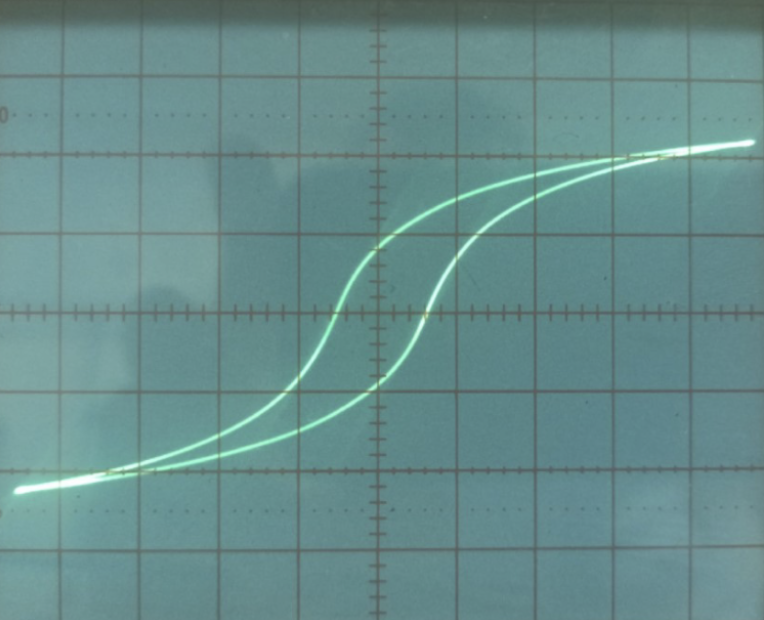
\includegraphics[width=0.7\linewidth,center]{p3.png}
    \caption{Схема экспериментальной установки}
    \label{fig:my_label}
\end{figure}
